\documentclass[fontsize=11pt]{article}
\usepackage{amsmath}
\usepackage[utf8]{inputenc}
\usepackage[margin=0.75in]{geometry}
\usepackage{graphicx}
\usepackage{indentfirst}
\usepackage[
backend=biber,
style=alphabetic,
]{biblatex}
\addbibresource{refs.bib}
\graphicspath{ {./images/} }

\title{CSC111 Project: Decoding the Secrets of Successful Stocks}
\author{Yehyun Lee, Aung Zwe Maw, Wonjae Lee}
\date{April 1, 2023}

\begin{document}
\maketitle
\section{Problem Description and Research Question}

\subsection{Project Goal}
As an investor, the question is, \textbf{which stocks are most profitable in the long-term, and what factors contribute to their success? Our team will use a tree data structure to identify the promising factors and the most likely companies to invest in and utilize the backtesting approach to determine the profitability of the investments.}
\\

We aim to determine the most promising stocks for investment by analyzing the correlation between their performance metrics. Based on the analysis, we will rank the stocks using a binary tree to group the stock by ranking for investment. We will then use the recommendation tree and invest according to what it suggests and draw conclusions on its performance.

\subsection{Motivation}
One of the reasons for this project is the increase in interest in stocks during and after the pandemic. Many people have turned to invest in stocks to make passive income or grow their savings during a time of economic uncertainty. However, with so many companies to choose from, it can be challenging to know which ones are most likely to provide a good return on investment. 
By using past datasets, we can analyze historical data, current market trends, and other relevant factors to identify the companies that are confused to perform well in the future. \\
This can help investors make more informed ed decisions about where to put their money and maximize their returns. Another motivation for developing a stock market investment program is the passion of one of our partners, Yehyun Lee for stock market trends. His passion positively affected us and we were also willing to explore the trends along with him.

\subsection{Context \& Required Knowledge}
Some background knowledge is required to understand the problem our team will be investigating. Stock investment involves buying and selling shares of companies with the expectation of earning a profit. When considering which stocks to invest in, that stores typically consider a range of factors, such as the price-to-earnings (PER), price-to-book ratio (PBR), and return on equity (ROE). These are three important factors.\\

PER can be calculated by share price / earnings per share. PBR is a company’s stock price / book value per share. The book value of a company is calculated as its assets minus its liabilities. In general, lower PER and PBR indicate how undervalued or cheap the price is; whereas higher indicates how overvalued or expensive the price is.\footnote{Further information regarding PER and PBR can be found in Appendix 6.1}\\

ROE measures profitability by calculating the amount of net income generated for each dollar of shareholder equity. A high ROE indicates that a company is generating significant profits for its shareholders, while a low ROE suggests that the company is not using its resources efficiently.\footnote{Further information regarding ROE can be found in Appendix 6.2}
\\

Please note that there will be more factors our team will use to identify hidden factors that influence stock performance.\footnote{Further information regarding other possible factors can be found in Appendix 6.3}
\section{Computational Overview}
\textbf{General Architecture, Function, Data Type and Algorithm}



For simplicity, we have split our code into fives files: main.py, part1\_user\_input\_visualization, part2\_factor\_processing, part3\_recommendation\_tree and part4\_investment\_simulation. Since, we want our program to run in a browser window using Streamlit, running our program calls the main.py file which in turns calls part1\_user\_input\_visualization which contains the Streamlit modules. Then this file in turn calls the part2\_factor\_processing, part3\_recommendation\_tree and part4\_investment\_simulation. \\

The part2\_factor\_processing will take in all the top performing stocks using the Yahoo Finance API \cite{jecsandyahoo}. This part of the program determines which factors are the most important for determining what stocks to invest in (Data for factor value is taken by Macrotrends). It will return the factors in order of least important to most important by calculating average correlation values (Further information can be found in 2.1).\\

The part3\_recommendation\_tree contains a binary tree data structure and takes the input of the factors and their correlation values from part2\_factor\_processing and builds a binary tree in with in order of least important to most important factors. This module contains a custom binary tree data structure with additional methods such as add\_subtree, insert\_stock and many more (Further information can be found 2.2). The generated tree is inserted with a list of all user input stocks. This tree helps classify which stocks to invest in according to risk percentage. \\

The part4\_investment\_simulation invest these stocks from the start year specified by the user until most recent year e.g. 2023. Then, a graph of return on investment is given as output to part1\_user\_input using the plotly function (Further information can be found 2.3) \\

The part1\_user\_input takes the plotly output given by part4\_investment\_simulation and plots these in a browser using Streamlit. It also allows for users to input directly in the browser instead of using the terminal (Further information can be found 2.4). Below is a brief diagram of general architecture and it will make more sense if you read with code in part 1 run\_program function.

\begin{center}
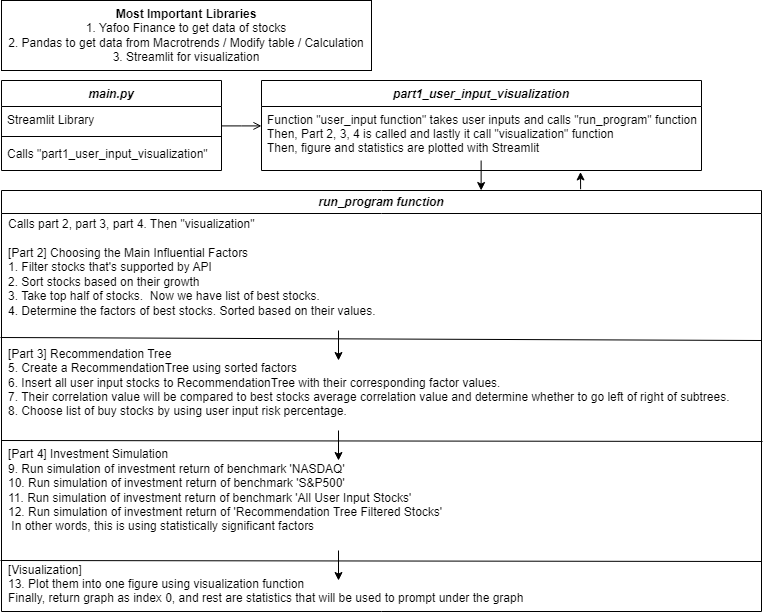
\includegraphics[scale=0.5]{CSC111.drawio.png}
\end{center}

\subsection{Choosing main influential factors - part2\_factor\_processing}
To calculate future investment stock returns, one of the foremost things to do is to get the dataset. This dataset would be obtained from “yahoofinancials” \cite{jecsandyahoo}, which is an Open Source, MIT Licensed library that uses an API to retrieve numerous information about the stock market from Yahoo Finance \cite{yahoofinancials}and also contains a variety of useful methods. Additionally, we will utilize a dataset from “Macrotrends”\cite{macrotrends}, a research platform that enables users to screen and research stocks and global metrics. We obtained further datasets up to 2009 by using the Pandas library\cite{pandas} and its’ “read\_html()” function. We have found a tutorial regarding the extraction of data on a website written by Medium \cite{tballz2022retrieving}.\\

This part of module will filter out stocks does not have sufficient data from Yahoo finance, then using data from 2009 to the user input date, it will calculate the percentage of growth and sort in order of performance. This is done by using one of the yahoofinancials methods which is `get\_percentage\_growth'. This function  that takes in the a stock name, start and end date and then returns how much the stock grew as float value. After sorting the stocks in order of their growth, the `top\_half', function is used to cut down the list of stocks ad select the top performing stocks.\\

The next imperative is to first identify the factors that influence investment planning. To determine these factors, the past datasets of the top performing stocks are scrutinized. Then, the factors belonging to each stocks such as "POE", "ROI" and more will be examined. The Pearson correlation\footnote{Information on why Pearson correlation is chosen on Appendix 6.4} of the changes in these factors would be plotted against the increase of stock price per year for each of the chosen top performing companies. This will be done using a method of pandas\cite{pandascorr} called `corr' which takes the data frame and outputs a correlation value enabling us to evaluate the extent of correlation between each factor and the stock price.
This will be repeated for each top companies and the average correlation value of factors will be taken. Below are the images of the sample a dataset of a company and its various factors provided by the API. \textit{(Dataset may differ according to actual results)} \\

\begin{center}
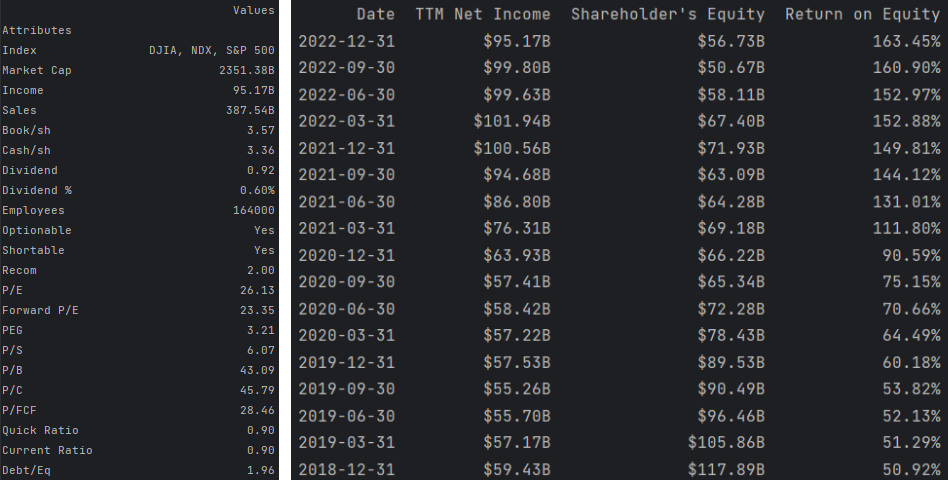
\includegraphics[scale=0.5]{dataset.png}
\end{center}

\subsection{Generating the Recommendation Tree - part3\_recommendation\_tree}
Now that the factors which are important is known, we have to create a recommendation tree. The algorithm for creating a complete recommendation tree is inspired by generate\_complete\_game\_tree from assignment 2, and it is customized to suit our RecommendationTree class. The recommendation tree is a tree data type that has four instance attribute: factor (string data type), left subtree (tree data type), right subtree (tree data type), correlation and list of stocks. The factor instance attribute stores the name of the factor which can be accessed while traversing the tree. Similarly, the correlation instance attributes stores the average correlation of each factor. The left subtree and right subtree are the left and right child of a parent tree. The list of stocks instance attribute is only used in the leaf nodes where the final list of stocks are stored after classifying. Below is a visual diagram of the a single tree node.\\

\begin{center}
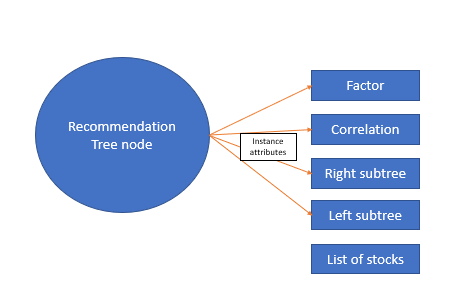
\includegraphics{tree_node.png}
\end{center}

The recommendation is tree is built by placing factors in a parent-child relation in the tree depending on the correlation value. For example, suppose the four factors are F1, F2, F3 and F4. F1 would be the parent of F2 if F1 has higher correlation of F2. F2 will be the parent of F3 if F2 has higher correlation value then F3 and so forth. Below is a diagram that demonstrates how a recommendation tree is built\\

\begin{center}
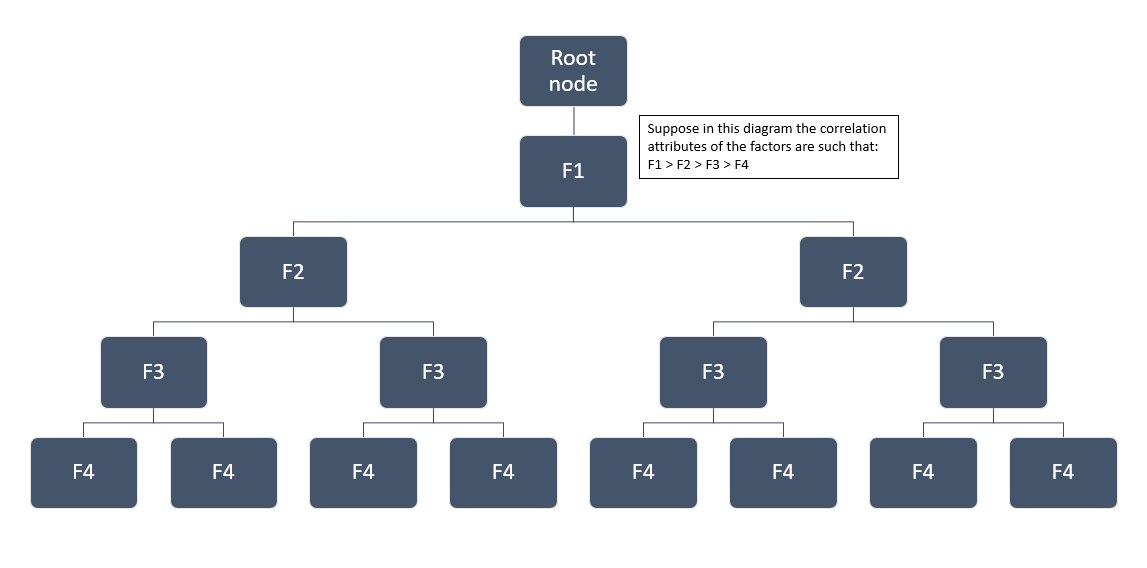
\includegraphics[scale=0.75]{tree_diagram.png}
\end{center}

Next, the values that would decide whether to invest in the company or not needs to be found. Suppose we are placing company A into the subtree. It gets inserted into the recommendation tree and arrives the F1 factor. 
To decide left or right, company A's F1 factor in correlation to stock price is taken. If the F1 factor correlation of company A is less than the average F1 correlation value, it traverses to left subtree. Otherwise, it goes into right subtree. Company A now arrives at the second intersection, and repeats these same steps and would repeat this process until it arrives at a leaf. This tree diagram allows for easier classification when choosing the optimal company to invest in. Below is a sample diagram how this classifying function works:
\begin{center}
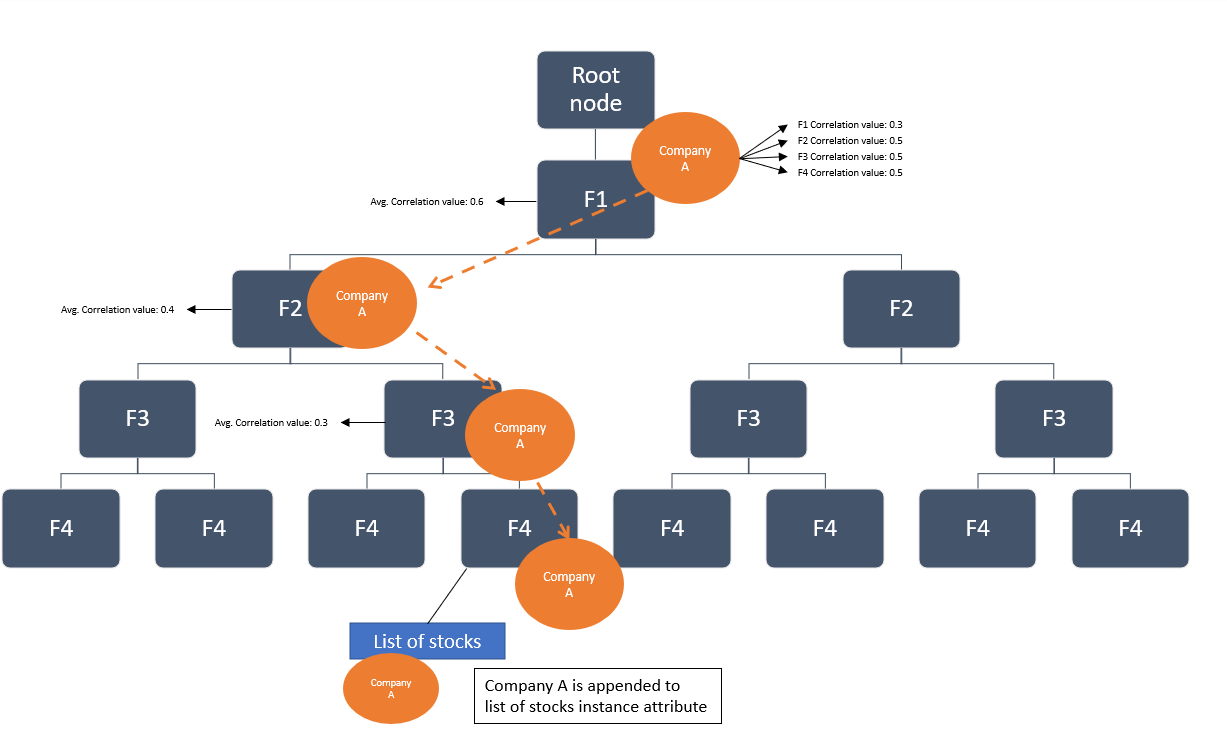
\includegraphics[scale=0.75]{tree_traversal.png}
\end{center} 
\subsection{Choosing the Stocks - part3\_recommendation\_tree}
With all the user input companies, the tree diagram would append them to a list in order of left to right. After all this is done, we call a function that gets appends all the list of stocks in the leaf nodes into  a list (therefore the output is a list of lists). For simplicity, let's assume this output as a variable name `All\_stocks'. Next another function would take the risk percentage and multiply it by the length of `All\_stocks' and rounds it up. Assume this variable as `i'. Finally, the program chooses the number of `i' elements starting from the right of `All\_stocks' A diagram of this process is attached below for better visual clarity:
\begin{center}
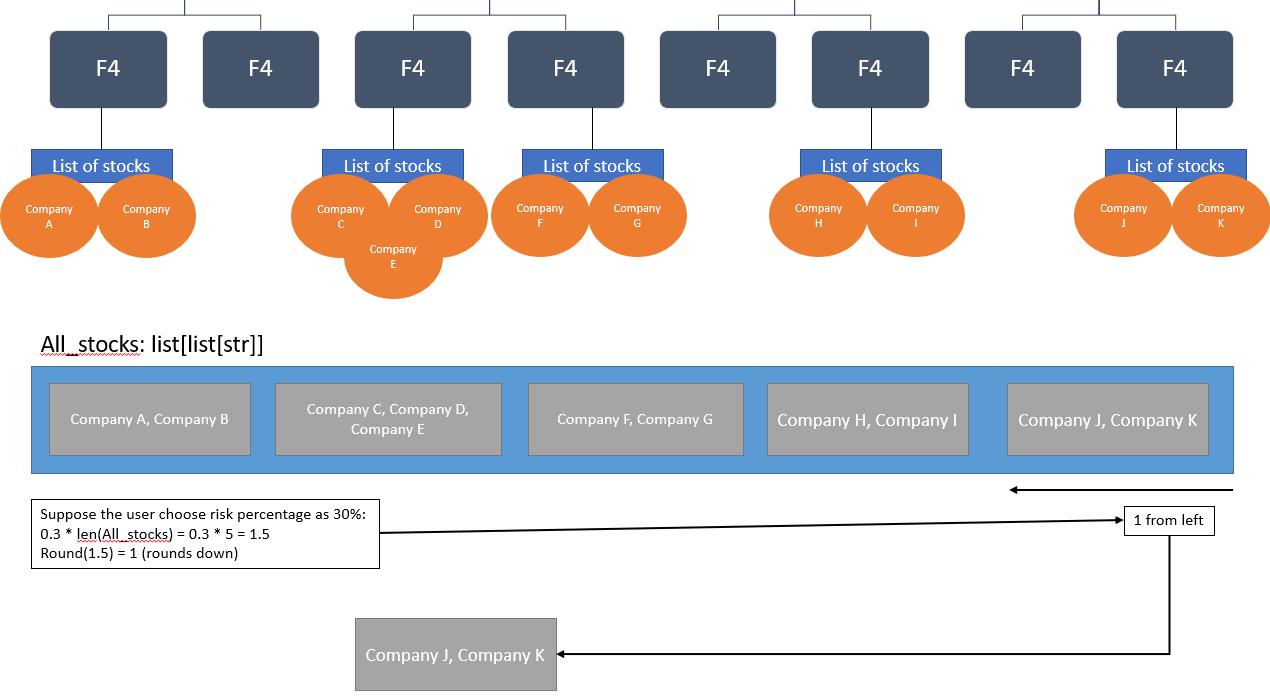
\includegraphics[scale=0.65]{choosing_stocks.png}
\end{center}
*At this point, you can assume the most far right is our top choice and the far left is the worst list of stock. In this example, the program will invest in Company J, K.

\subsection{Simulation - part4\_investment\_simulation}
The selected stocks are then invested from the starting date provided  given by the user during part 4. Then a function called `recommendation\_tree\_simulation' invests them starting from the date given by the user until the current year which 2023. It then outputs the values a dictionary where the keys are the number of years and values are the percentage return over investment. Next, we need a comparison to understand how good our function is. Hence, another function called `benchmark\_simulation' is made which invests in takes input a list of stocks and outputs its keys as the number of years and values as percentage return over investment. 
This function `benchmark\_simulation' is used to run the original list of stocks the user gave, as well as the NASDAQ and S\&P500. In comparison, the recommendation tree only invests in what is determined as `good stocks' from the list of stocks given by the user. The values of all these three as well as the output from `recommendation\_tree\_simulation' is then plotted as line chart which is figure data type.

\subsection{Visualization - part1\_user\_input}
The Streamlit library is in a separate file called `part1\_user\_input\_visualization'. This module is solely responsible for running functions from part 2, part 3 and part 4 and then getting the line chart as figure data type. This is then displayed in a browser. One of the reasons of using Streamlit is that it allows for users to input values directly from the browser and the user can simply click `Run Program'. Please refer to \textbf{Section 3: User Instructions} for more details about the graph. Additionally, PIL library has to been imported to allow images to be displayed in the browser. 

\section{User Instructions}
Firstly, download all required libraries from the requirements.txt. Then, run main.py. If the user is running Streamlit for the first time, Streamlit will prompt you to enter an email address to receive newsletters as shown in the image below. 
\begin{center}
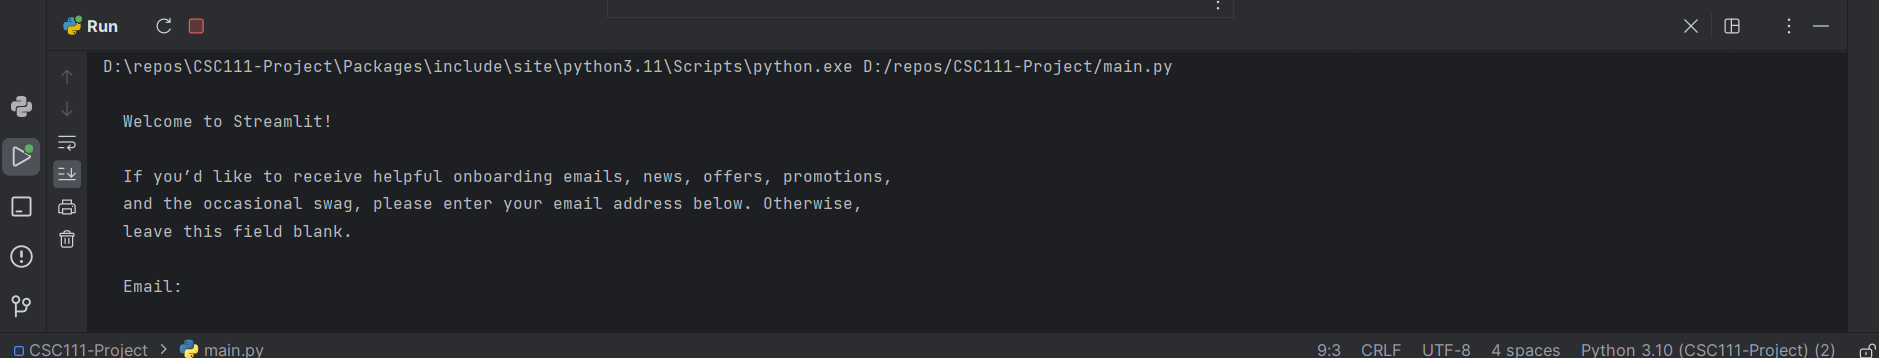
\includegraphics[scale=0.27]{streamlit_prompt.png}
\end{center} 
Skip this by clicking enter. User might also get a prompt to allow firewall permissions. Just leave it on default and click on `Allow access'. 
\begin{center}
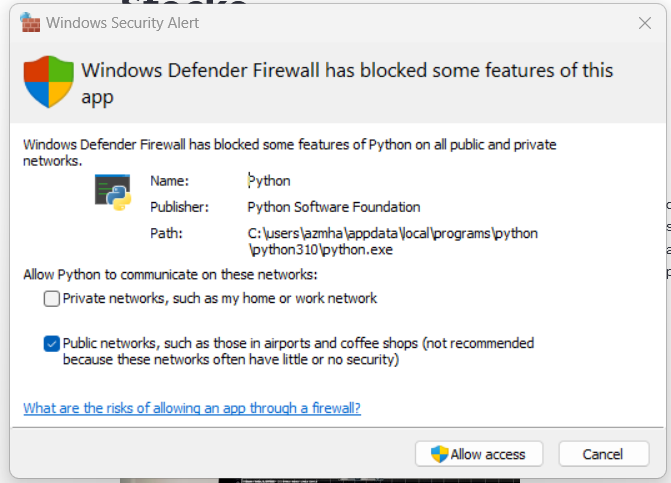
\includegraphics[scale=0.5]{firewall.png}
\end{center}
This will open up a browser that allows the user to input values and run the simulation. The user should choose a list of stocks, start date, risk percentage, and factors. For the list of stocks, as explained in \textbf{Section 4.2}, user can run as auto, options (that allows users to choose stocks from the drop down menu) and manual (that allows users to manually type stocks). We highly recommend avoiding using the manual option. Use either auto or options. If you are running with check\_contracts, choose a small number of factors, as many factors lead to a significant increase in running time due to the nature of the Recommendation Tree. Without check\_contracts you can select all without worrying about running time. We recommend you comment out python-ta while running Streamlit, if not, it will keep open up the python-ta due to Streamlit refreshing. After all the required values are given, click on `Run Program' button and Streamlit should return the results in approximately 5 minutes. Note that pressing the \textbf{run button once is enough}. Pressing it multiple will cause the program to rerun again which would result in even longer run times. The program is also coded to run with default values in the case of the user forgetting to specify a variable. \textbf{Please ensure that the user has a stable internet connection}. If a decent internet connection is not established the function will not run and may cause errors. The images below show the errors that the user will encounter without a proper connection. 
\begin{center}
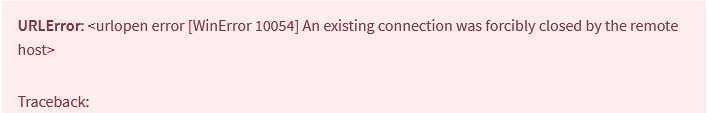
\includegraphics[scale=0.65]{error.png}
\end{center}
With a proper connection, the user will see a graph being displayed. The graph for display by the Streamlit outputs four distinct lines. It will show the return over investment for S\&P500 and NASDAQ. It will also show what happens if user buys all stocks in the given as the input represeted by the `All User Input Stocks' line. The line shown as `Recommendation Tree Filtered Stocks' is the return over investment of what happens if the user input a list of stocks but the program only invests in what it determines to be `a good stock'.\\

Here's what our program looks like when we input selecting all stocks, default date, risk percentage of 1, and all factors. It performs better than the S\&P500 because it only takes the best-performing stocks based on their correlation value and invests in them. The program will also prompt ranked factors such that the user can identify which factors were secrets of successful stocks:

\begin{center}
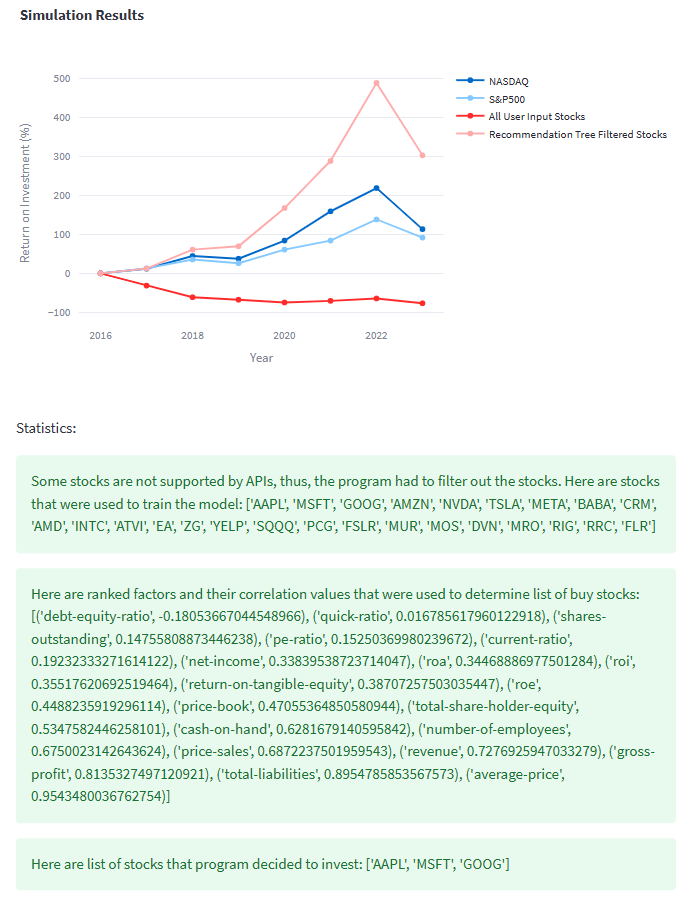
\includegraphics[scale=1]{visualization.png}
\end{center}

\section{Changes Made to the Initial Proposal}
\subsection{Regarding data processing and calculations}
In our first proposal, we mentioned  using standard deviation to obtain a correlation value for each factor which would help determine whether the recommendation tree would traverse to the left or right subtree. We decided against this and only took average values instead because standard deviation assumes the normal distribution pattern in the values. Our correlation values are obtained but examined the factors with top companies and does not have much to do with the normal distribution pattern. 

\subsection{User Input}
Second, we have changed what our user input would be for the function determining\_buy\_stocks. Originally, our idea was to have an input called `range of leaf nodes' which the user would input a number that would determine the range of leaf nodes chosen. However, through our simulations and testing, we found that for our submission, we changed our input and called it `risk percentage'. The reason is because we would not have to limit this user input since we can calculate which stocks to choose based on the Recommendation Tree as the number of leaf nodes is dependent on the number of factors of user chooses. \\

User input was also slightly modified where in the original, the user is solely responsible in entering the list of stocks to invest, the number of years and factors they chose. However, we realized that we actually do not know the amount of knowledge the user has about the stock market. Therefore, we slightly modified the inputs by adding default options allow user to run in the `Auto' mode where the a pre-selected list of stocks is available for the users to directly run. In good\_bad\_stocks.csv, we included around half companies with good stock and another half of companies with bad stock to have a balanced list of stocks of good and bad. Users can choose to use this list of stocks. We also have an `Option' mode where user can select a multiple stocks from a drop down menu. Finally, for users with expertise in the stock market, we included a manual mode where a company's stock name can be typed manually. \\

Another input we removed was the investment amount because we would like the user to understand how much return they are making. If investment amount was included just by returning the amount made, the user's perception on how much profit might be influenced by how much they initially invested. Therefore, by removing the investment amount and just returning the percentage of return over investment, we area able to present a better picture of how much profit is made to the user.
\subsection{Changes to Simulation}
In the previous proposal, we decided to run the recommendation tree each year for the number of years given by the user. Then, we would buy and sell every year according to the recommendation diagram. Below is what we initially proposed:
\begin{center}
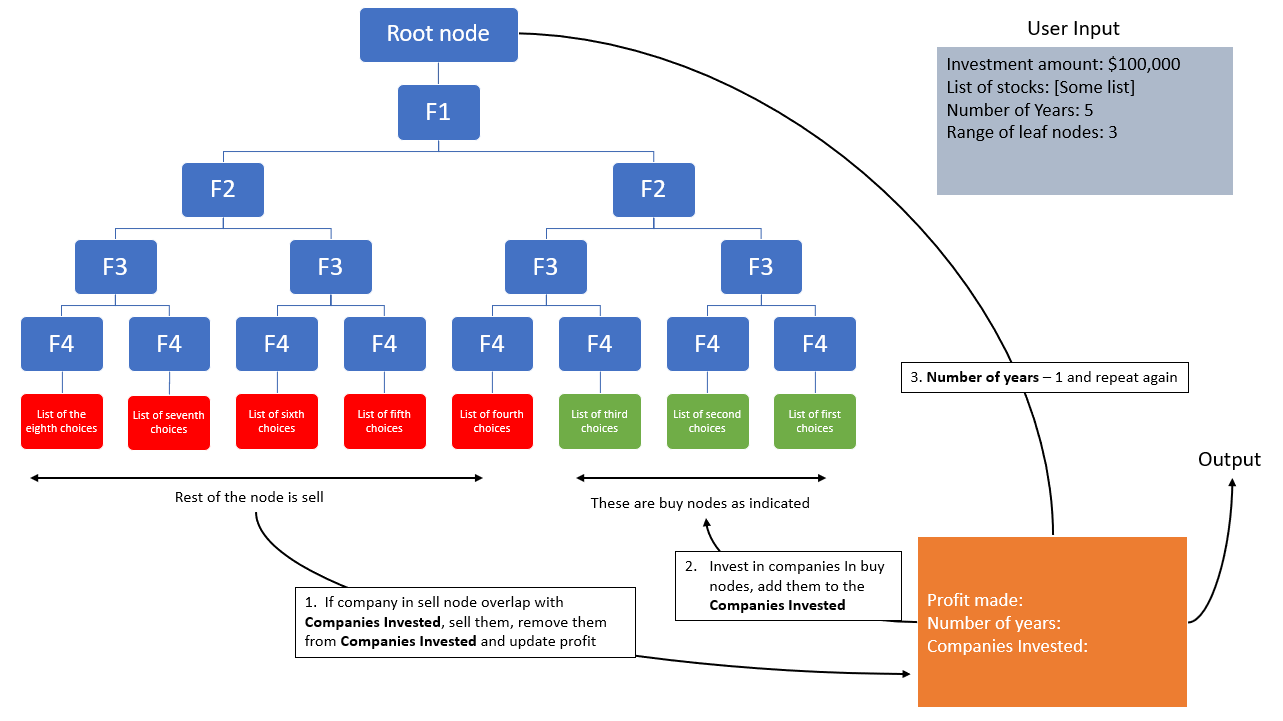
\includegraphics[scale=0.65]{ai_diagram.png}
\end{center}
After much of testing and simulation we decided that we would only run the program once during the initial year of investment (given by the user) to determine which stocks to buy and hold these stocks for until the current year instead of buying and selling each year. This was agreed after a long discussion with group members as it would be a better representation of whether our program performs well or not.
\section{Discussion}

\subsection{Goals and Insights}
Our team successfully used a tree data structure to identify the promising factors and the most likely companies to invest in and utilize the backtesting approach to determine the profitability of the investments.\\

We explored the question: which stocks are most profitable in the long-term, and what factors contribute to their success? Based on the result of the simulation, we were able to determine the most promising stocks for investment by analyzing the correlation between their performance metrics. Thus, we were able to find the secrets of successful stocks by studying factors' correlation values using a tree data structure.\\ 

The program ranks the stocks using a binary tree to group the stock by ranking for
investment. Then it uses the recommendation tree and invests according to what it suggests and draws conclusions on its performance. As an example, it performs better than the S\&P500 as it only takes the best-performing stocks based on their correlation value and invests in them. 
 Then, it prompts the factors in ranked order, enabling users to identify what factors contribute to their success. From the simulation results image from page 9, based on that one example, we can determine that `average-price' had a 0.95 correlation value, meaning `average-price' above 0.95 is a strong sign of good stock. Other factors like  `total-liabilities', `gross-profit', `revenue' also had a statistically significant  contribution to the success of stocks, and that `AAPL', `MSFT' and `GOOG' are the ideal stocks to invest in.
 \\
 
After a series of debugging and extensive testing done to the program, we came to a few conclusions regarding the program. Our program compares the current trends of stock market and invest accordingly which means a user investing with our program will not be experience significant risks. However, sudden disruptions would greatly affect the profitability of our program. An example of this would be the COVID-19 pandemic. Our program saw significant decrease in profit and sometimes even losses during the years between 2019 - 2021 as it was not able to predict most viable stock to invest in the pandemic era by just using previous trend data.

\subsection{Limitations and Obstacles Encountered}
One obstacle we encountered was our data was shown originally. When extracting data from the Macrotrends website, we found out there was unnecessary data being shown that would slow down our program. We overcame this with our `obtain\_factor\_data' and `clean\_and\_merge' functions. After extracting our data and adding it into a Pandas dataframe, we isolated which parts of data we wanted by using indexing and try and except for errors. While working on finding the correlation by using the merge function, it would return an empty dataframe. This occurrence happened because some of the data was blank or NaN. Our solution was to use the function `dropna'. We also had issues with pandas' read\_html() function. The try and except function that we wrote for our function did not work. An additional import `from lxml import etree' had to be imported to catch pandas' read\_html() errors.
\\

At one point, we considered using only Plotly for our plotting, but we wanted to have the user be able to add or remove inputs and the graph would update in real time. We realized that Plotly by itself does not have the capabilities to do what we wanted. Ultimately, we figured out Streamlit was a good option for our plotting but we later realized that the user has to run commands into cmd when running Streamlit. 
\\

Another problem we encountered was the python-ta's check\_contracts. Before adding check\_contracts to our RecommendationTree class, we had no issues. However, while testing RecommendationTree after adding check\_contracts, we encountered AssertionErrors. The error claimed that our return value did not match the return type annotatiton even when it did. After some enquiries, our Professor advised that the typeguard library is the issue. To fix our problem, we had to specify the typeguard library version to 2.13.3, not 3.0.x.
\\
Some stocks were not supported by the Macrotrends website and the Yahoo Finance library which caused issues. So we had to filter out the stocks that are not supported by either of them. Now everything is fixed withour errors when we run with check\_contracts.
\\

Python-ta caused many issues in which it would return an error message saying the `ClassDef' object has no attribute `value' and contact the instructor with code. We realized that using the iloc function from pandas was causing this error so we decided to use the filter function instead.

\subsection{Further Exploration Options}
After testing and running our program, the project has shown promising results. One method to expand our project is to run our program to actually buy stocks from the stock exchange instead of a simulation. We can have the AI buy, hold and sell stocks every year and see the long-term results. However, before implementing this, we would need to extensively test out our program and ensure that losses are not made. Additional inspections must also be made to ensure that our program is secure from malicious actors.\\

We can also make improvements with using APIs. APIs we used like Yahoo Finance and Macrotrends did not support some stocks and we had to handle error cases and drop NaN. Instead, we could look for better supportive APIs that will far better suit the project's purpose.\\

Lastly, we can make improvements with statistics results. If we're changing the program with AI deciding to buy, hold, and sell every year, we could've calculated the win/loss ratio, max drawdown, and more in-depth analysis of factors' correlation values.

\pagebreak
\section{Appendix}

\subsection{Regarding PER and PBR}
If PER means “how much this company earns and the stock price is this much”, PBR is the concept of “how much this company owns and the stock price is like this”.
\\

Some companies have a high PBR due to the nature of the industry.  Ex) Bio companies; since they do not need much land due to the nature of the research company. In addition, AAPL (Apple)  has a high PER and PBR, not because it’s an indication of a bad company, but it’s an indication of AAPL being an expensive stock. So PER and PBR don’t always indicate whether the company is bad or not.

\subsection{Regarding ROE}
ROE is what Warren Buffet—world’s greatest investor—enjoys using. He advises investing in companies with a ROE of 15\% or higher and steadily increasing within the last three years \cite{investopediawarren}.
\\

ROE or the return on equity can be calculated by net income / shareholder’s equity.

\subsection{Additional Factors}
Some other factors that might be important are dividend yield, debt-to-equity (D/E), profit margins, etc. Dividend yield is also one of the important factors. It measures the amount of cash dividends distributed to shareholders in relation to market value per share. This is used to evaluate the income potential of a stock investment. Higher is better for investors.

\subsection{Regarding Mathematical Analysis}
For the correlation, we have decided to use the Pearson correlation as we are analyzing the linear correlations instead of the monotonic relation \cite{user3636user3636} \cite{machinelearningmastery}.

\printbibliography

% NOTE: LaTeX does have a built-in way of generating references automatically,
% but it's a bit tricky to use so we STRONGLY recommend writing your references
% manually, using a standard academic format like APA or MLA.
% (E.g., https://owl.purdue.edu/owl/research_and_citation/apa_style/apa_formatting_and_style_guide/general_format.html)

\end{document}
